%%%%%%%%%%%%%%%%%%%%%%%%%%%%%%%%%%%%%%%%%%%%%%%%%%%
%
%  New template code for TAMU Theses and Dissertations starting Fall 2012.  
%  For more info about this template or the 
%  TAMU LaTeX User's Group, see http://www.howdy.me/.
%
%  Author: Wendy Lynn Turner 
%	 Version 1.0 
%  Last updated 8/5/2012
%
%%%%%%%%%%%%%%%%%%%%%%%%%%%%%%%%%%%%%%%%%%%%%%%%%%%

%%%%%%%%%%%%%%%%%%%%%%%%%%%%%%%%%%%%%%%%%%%%%%%%%%%%%%%%%%%%%%%%%%%%%%
%%                           SECTION I
%%%%%%%%%%%%%%%%%%%%%%%%%%%%%%%%%%%%%%%%%%%%%%%%%%%%%%%%%%%%%%%%%%%%%


\pagestyle{plain} % No headers, just page numbers
\pagenumbering{arabic} % Arabic numerals
\setcounter{page}{1}


\chapter{\uppercase {Introduction and Background}}

Seismic reflection is the most important method used in the oil \& gas exploration industry. Huge amount of seismic data has already been generated and processed for several decades in such area, although there was no such big data concept at that time. In seismic data flow such as acquisition, migration and interpretation, it involves a lot of domain-specific specialists and computer scientists to work together. Since the seismic data processing is both computation- and data-intensive, the High Performance Computing (HPC) technology was widely used in this area; The typical working flow should be: geophysicists use MATLAB to verify algorithms on small or synthetic sample data, then submit verified algorithms to computer scientists who will translate them into MPI codes that could run efficiently with actual data on cluster. Such procedure is both time-consuming and high-stakes that need much communication and iterations due to premature design or inconsistent results on sample and actual data. With the improvement of the data acquisition methods and requirements of high resolution for advance processing algorithms, the volume size of seismic data increases drastically, which is big challenge for the traditional way. In this paper, we will try to setup a seismic data processing platform on which all stakeholders could work with same data sets and algorithms or models without much performance expense.

\section{Seismic Data Processing Flow}
As a dominant method of exploration geophysics in oil \& gas area, reflection seismology (or seismic reflection) uses the principles of seismology to estimate the properties of the Earth's subsurface from reflected seismic waves \cite{seisreflectionwiki}. Although the theory of reflection is simple, but the processing flow is more sophisticated in practical scenario. The main steps in such work flow include: data acquisition, data processing, data interpretation and attribute analysis.

In the data acquisition stage, seismic sources such as dynamite or air gun are used to generate seismic waves, and the waves are reflected or refracted while encountering different type of materials underground and are recorded by the receivers. It becomes more complicated in non-normal incidence, such as refraction, multiple reflection and cultural noise, and all these factors need to be considered in processing stage. The first stage is pre-processing after acquiring the survey data, in which main steps are removing noise and boosting signal level. Velocity analysis, stacking and migration are main tasks in seismic data processing, and after migration the seismic events are geometrically re-located in either space or time to the location the event occurred in subsurface and create a complete image of subsurface \cite{seisreflectionwiki}. The main goal of seismic interpretation is trying to find petroleum reservoir. But such task requires deep analysis of seismic attributes and geophysics related knowledge, and involves huge amount human resource such as computer scientists, geologists and geophysicists etc. In this paper, we focus on latter stage and built a platform that facilitates seismic attributes extraction and analytics.   

\begin{figure}[h]
\centering
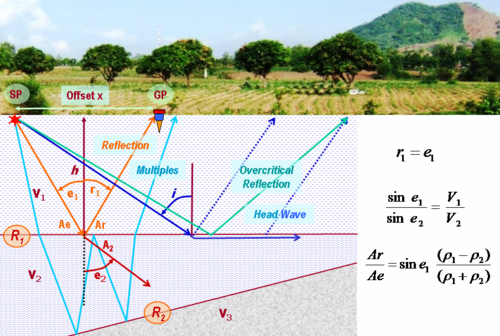
\includegraphics[scale=0.4]{figures/seismic_reflection_principal.png}
\caption{Illustration Seismic Reflection \cite{seisreflectionepa} \cite{seisreflectionagile}}
\label{seismic_reflection}
\end{figure}

%A landscape figure should be shown below. 
%%%%%%%%%%%%%%%%%%%%%%%%%%%%%%%%%%%%%%%%%%%%%%%%%%%%%%
%\begin{sidewaysfigure}[H]
%\centering
%
\includegraphics[scale=.50]{figures/Penguins.jpg}
%\caption{TAMU figure - This is an example of a long figure title with a landscape figure.  Figure titles need to be single-spaced within and double spaced between in the list of figures.}
%\label{fig:tamu-fig1-1}
%\end{sidewaysfigure}
%%%%%%%%%%%%%%%%%%%%%%%%%%%%%%%%%%%%%%%%%%%%%%%%%%%%%%


\section{Current Processing Methodlogy}
HPC technology has been used to process seismic data for several decades. In most current big oil \& gas companies or related service companies, there must have an IT department and a huge group of geophysicists or data scientists forming the research teams. In normal case, each small team set up a research project, and then develop new models or algorithms to verify their idea. In this stage, they only use synthetic or historical small data to do experiments, and their programming environment is MATLAB in general. But why did not they develop algorithms and models on big cluster with actual seismic data? The main reason is that geophysicists are not familiar with HPC environment, and their main target is to verify the validity of algorithms\/models, but not the performance. The volume size of actual data is usually very large and will take much more time to run with MATLAB codes. After research work was finished and got approval, geophysicists will submit their MATLAB codes to IT department, and then experts in HPC domain will translate such codes into MPI codes or hybrid OpenMP/MPI codes and verify them on high performance cluster with actual seismic data. If there are any problems in such stage, the original authors need to be involved to find the root cause together, and the results were either changing algorithms\/models by geophysicists or modification of programming implementation. To make such a research project become a mature product, it will often take one more year with several iterations.

%\subsection{This is a Very Long Subsection Title This is a Very Long Subsection Title}


\section{The Facing Challenges}

\subsection{Problems of Existing Solution}
In fact, there are problems in current seismic data analytics flow. As shown in previous section, the MATLAB codes work well on sample data do not mean they could run successfully in parallel after translating into MPI codes. The test cases on MATLAB codes are usually not enough, and the parallelization itself may also produce new problems.
Another problem is the maintenance and reuse of legacy codes; Most of HPC codes in such area were written in Fortran to achieve high performance, the readability and maintenance of such programs are also challenges for beginners or successors. With the improvement of CPU computation power and programming architecture, we should not only focus on execution time, but also the overall performance of whole company and entire industry. 

\subsection{New Challenge from Big Data}
Currently, almost every industry could not live without network. With network including Internet, the data scattered everywhere could be transferred and be integrated for processing and analysis, and then form the basis for some new business such as search engine, social network and E-commerce etc. With the boom of social network, everyone becomes a media source instead of traditional centralized media portal, and the transaction data of online shopping increase drastically in recent years. Besides these popular area, some new direction such Internet of Thing (IoT) also grows quickly, so the big data has already been generated and will continue increase exponentially, which is big challenge for every industry.    

Big data \cite{WikiBigData} is a broad term for data sets with large volume,complex variety and high velocity which could not be handled by traditional data processing applications. The biggest challenges in seismic domain from now on are burst increase of acquired data volume size and high-speed streaming data from sensors in well need to be analyzed on time. Conventional RDBMS could not store wide variety data obviously, and moreover, different types of data from exploration, simulation and well logs need to be analyzed jointly, which also need more advance algorithms and models to process. For instance, the volume size of high dimension such as 3D even 4D seismic data and high density seismic data are growing exponentially, so seismic data processing becomes both computation- and data- intensive problems. The traditional HPC programming model is good at handle computation intense case, but for huge increase of volume size, data movement between nodes is the greatest bottleneck even with InfiniBand connections. In summary, oil \& gas domain also facing the big challenges including data storage, transfer, analysis and visualization etc.

